\section{模型假设及适用范围}

\subsection{全题共用的模型假设}

为使各问采用一致的空间与能量计算口径，并避免引入附件未给出的参数，作如下四条假设。货箱不可拆分、返航安全余量等题设要求属于约束条件，不在此重复列为假设。

\begin{figure}[H]\centering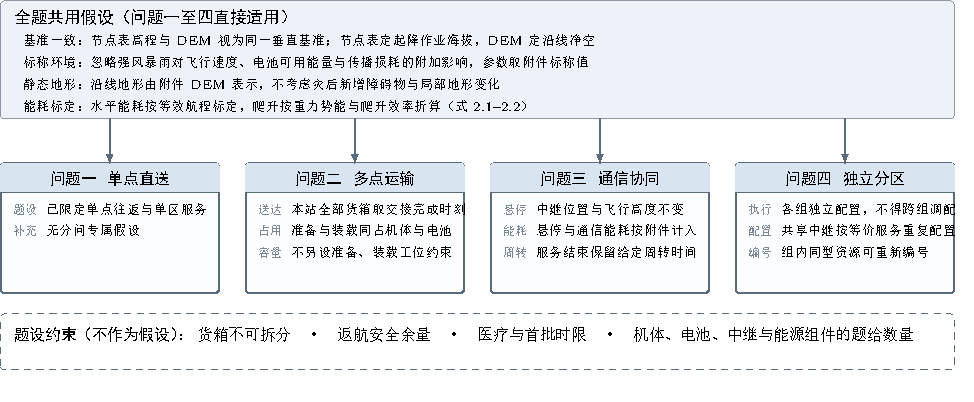
\includegraphics[width=\textwidth]{../figures/fig_assumption_scope.pdf}\caption{模型假设的适用范围：全题共用假设、分问补充口径与题设约束}\label{fig:assumption_scope}\end{figure}

（1）垂直基准一致。假定节点表中的地面海拔与数字高程模型（DEM）采用相同的垂直基准，可据此比较节点作业海拔与沿线地形高程。题目要求两类数据共同确定巡航海拔和通信端点位置，却未给出基准转换参数，故以一致基准作为高度计算的前提。实测显示，节点表高程与对应DEM像元高程的最大绝对差约10.56~m，因此本文不把两者混用：以节点表确定起降作业海拔，以DEM确定沿线净空与遮挡，并保留两套原始值。该假设影响爬升高度、运输能耗、航段净空及地形遮挡判定；若发现系统性高程偏差，应先校正数据并重新检验方案。

（2）标称环境。在题设标准测试场景下，忽略强风、暴雨等极端天气对飞行速度、电池可用能量、耗电率及无线传播损耗的附加影响，直接采用附件给出的标称参数。附件未提供逐时风雨数据及参数修正关系，因而难以对上述影响作可复核的定量估计。这一简化可能使飞行时限、返航电量和通信连续性的可行性判断偏于乐观，故在敏感性分析中分别对速度、能耗与链路损耗作扰动检验；若实际环境超出无人机允许的运行条件，须重新规划任务。

（3）静态地形。假定规划期内航段沿线地形可由附件DEM表示，不额外考虑灾后新出现且未记录的障碍物或局部地形变化。题目仅提供一套地形数据，采用同一地形面可保证运输净空与通信遮挡判定的一致性；若滑坡堆积或临时设施使局部障碍高度显著变化，该假设可能低估碰撞及失联风险，应更新地形数据后重新计算相关航段与链路。

（4）能耗标定。以机型的单组电池可用能量与载荷对应的等效航程之比，标定该载荷下单位水平距离的运输能耗；爬升附加能耗按重力势能和爬升效率折算，即采用式~\eqref{eq:range}--\eqref{eq:energy}。题目给出这些参数及“水平能耗与爬升能耗之和”的结构，但未展开水平能耗公式，因此需确定这一可逐段核算的对应关系。该假设影响最大安全载荷、架次能量可行性及后续调度结果；返航安全余量在汇总架次能耗后单独检验，以避免重复扣减。

\subsection{各问题的补充约定与适用范围}

四个问题逐步增加资源、时间、通信和独立分区约束。为避免把题目规定误写成模型假设，下面只区分各问的题设边界与求解所需的补充口径，目标优先级与算法选择在各问模型中另行说明。

（1）问题一。题目已规定每个架次采用O01$\to$S$_i$$\to$O01的直接往返形式、每次只服务一个服务区，并暂不考虑实体无人机和共享电池的时序调度，故本问不再设置分问专属假设。其结果只反映不同机型在各服务区的安全载荷与货箱组批能力，可作为后续问题的运输能力基准，但不能说明多架无人机同时执行时的任务完成时间和资源可行性。

（2）问题二。对于同一服务区内由同一架次交付的多个货箱，统一以本站全部货箱完成交接的时刻作为其送达时刻；附件仅给出接收点基础交接时间和每箱增加时间，未给出箱内交接顺序，采用交接完成时刻可避免人为指定顺序，并对时限检验形成保守估计。准备和装载阶段同时占用执行无人机及所装电池，以防止同一资源在该时段被重复安排；由于附件没有给出准备、装载工位及地勤人员数量，不对不同无人机的地面作业附加互斥约束。若实际只有有限工位，则需增加相应容量约束，所得调度完成时间可能延长。

（3）问题三。假定每个中继架次到达选定悬停点并完成建链后，在相应服务时段内保持该水平位置和飞行海拔不变，服务结束后再返回O01。题目要求确定中继的悬停位置、飞行海拔与服务时段，并给出了悬停功率，因此固定悬停能够使链路状态、服务时间和能源消耗保持一致且可复核。该假设将中继决策限定为“位置—高度—时间区间”的组合；若允许中继机在服务期间随运输机移动，可能减少中继数量或扩大覆盖范围，但必须进一步建立移动轨迹、动态链路和附加飞行能耗模型。

（4）问题四。题目要求保持问题三既定的货箱组批、访问顺序、运输与中继任务安排及通信关系，并禁止资源跨组调配。若同一中继架次在问题三中为不同任务组的运输任务提供通信，则在独立执行条件下，各相关任务组均需配置与原任务等价的中继服务，不能继续共享同一实体或能源组件；组内同型资源允许重新编号，其需求量按固定任务时间区间的最大重叠数确定。该处理体现了“各组可独立完成任务”的要求，但会放大共享资源被分割后的重复配置成本；若允许跨组协同或重新优化任务时刻，资源需求需另行计算。
